%!TEX root = ../../../main.tex

\subsection{2D CNN based clip-level feature extraction}
    First, the ResNet-50 CNN \cite{he2016deep} is used as a 2D CNN network to extract spatial features of each frame in video.
    Figure \ref{fig:resnet50} illustrates the architecture of ResNet-50 which composes of five convolutional blocks stacked on top of each other.
    % The network is pre-trained on ImageNet then fine-tuned using training sets described in Section \ref{sec:experimental_result}.
    Deep residual features are extracted from the output of the last convolutional block of the network which is a 2048-D feature vector.
    \begin{figure}[htbp]
        \centering
        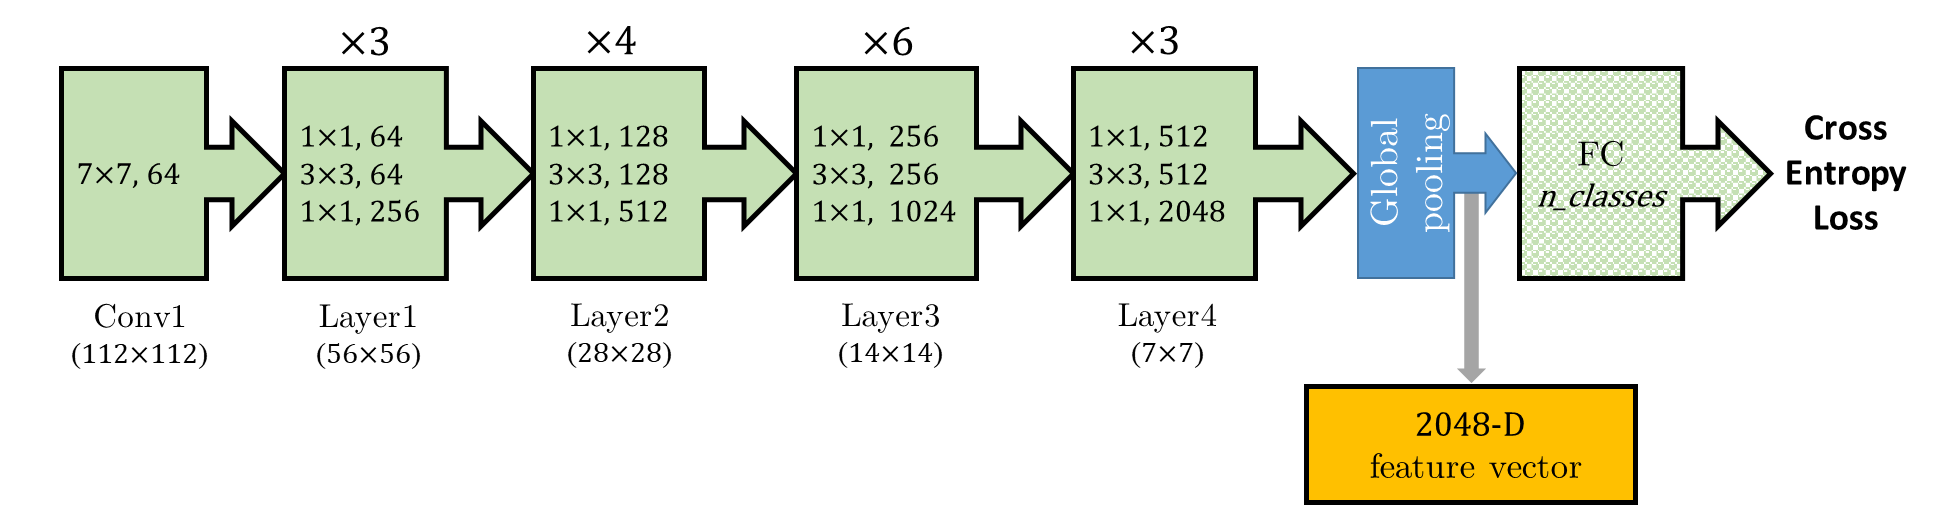
\includegraphics[width=1\linewidth]{figs/Resnet50.png}
        \caption{Architecture of ResNet-50 utilized in this work for feature extraction at each separated view.}
        %\vspace{-0.3cm}
        \label{fig:resnet50}
    \end{figure}
    After that, frame-level features are aggregated to create video-level features.
    In this work, three temporal modeling techniques are implemented: 1) average pooling (AP); 2) recurrent neural network (RNN) and 3) temporal attention (TA).
    Figure \ref{fig:pooling} illustrates three techniques.
    \begin{figure}[htbp]
        \centering
        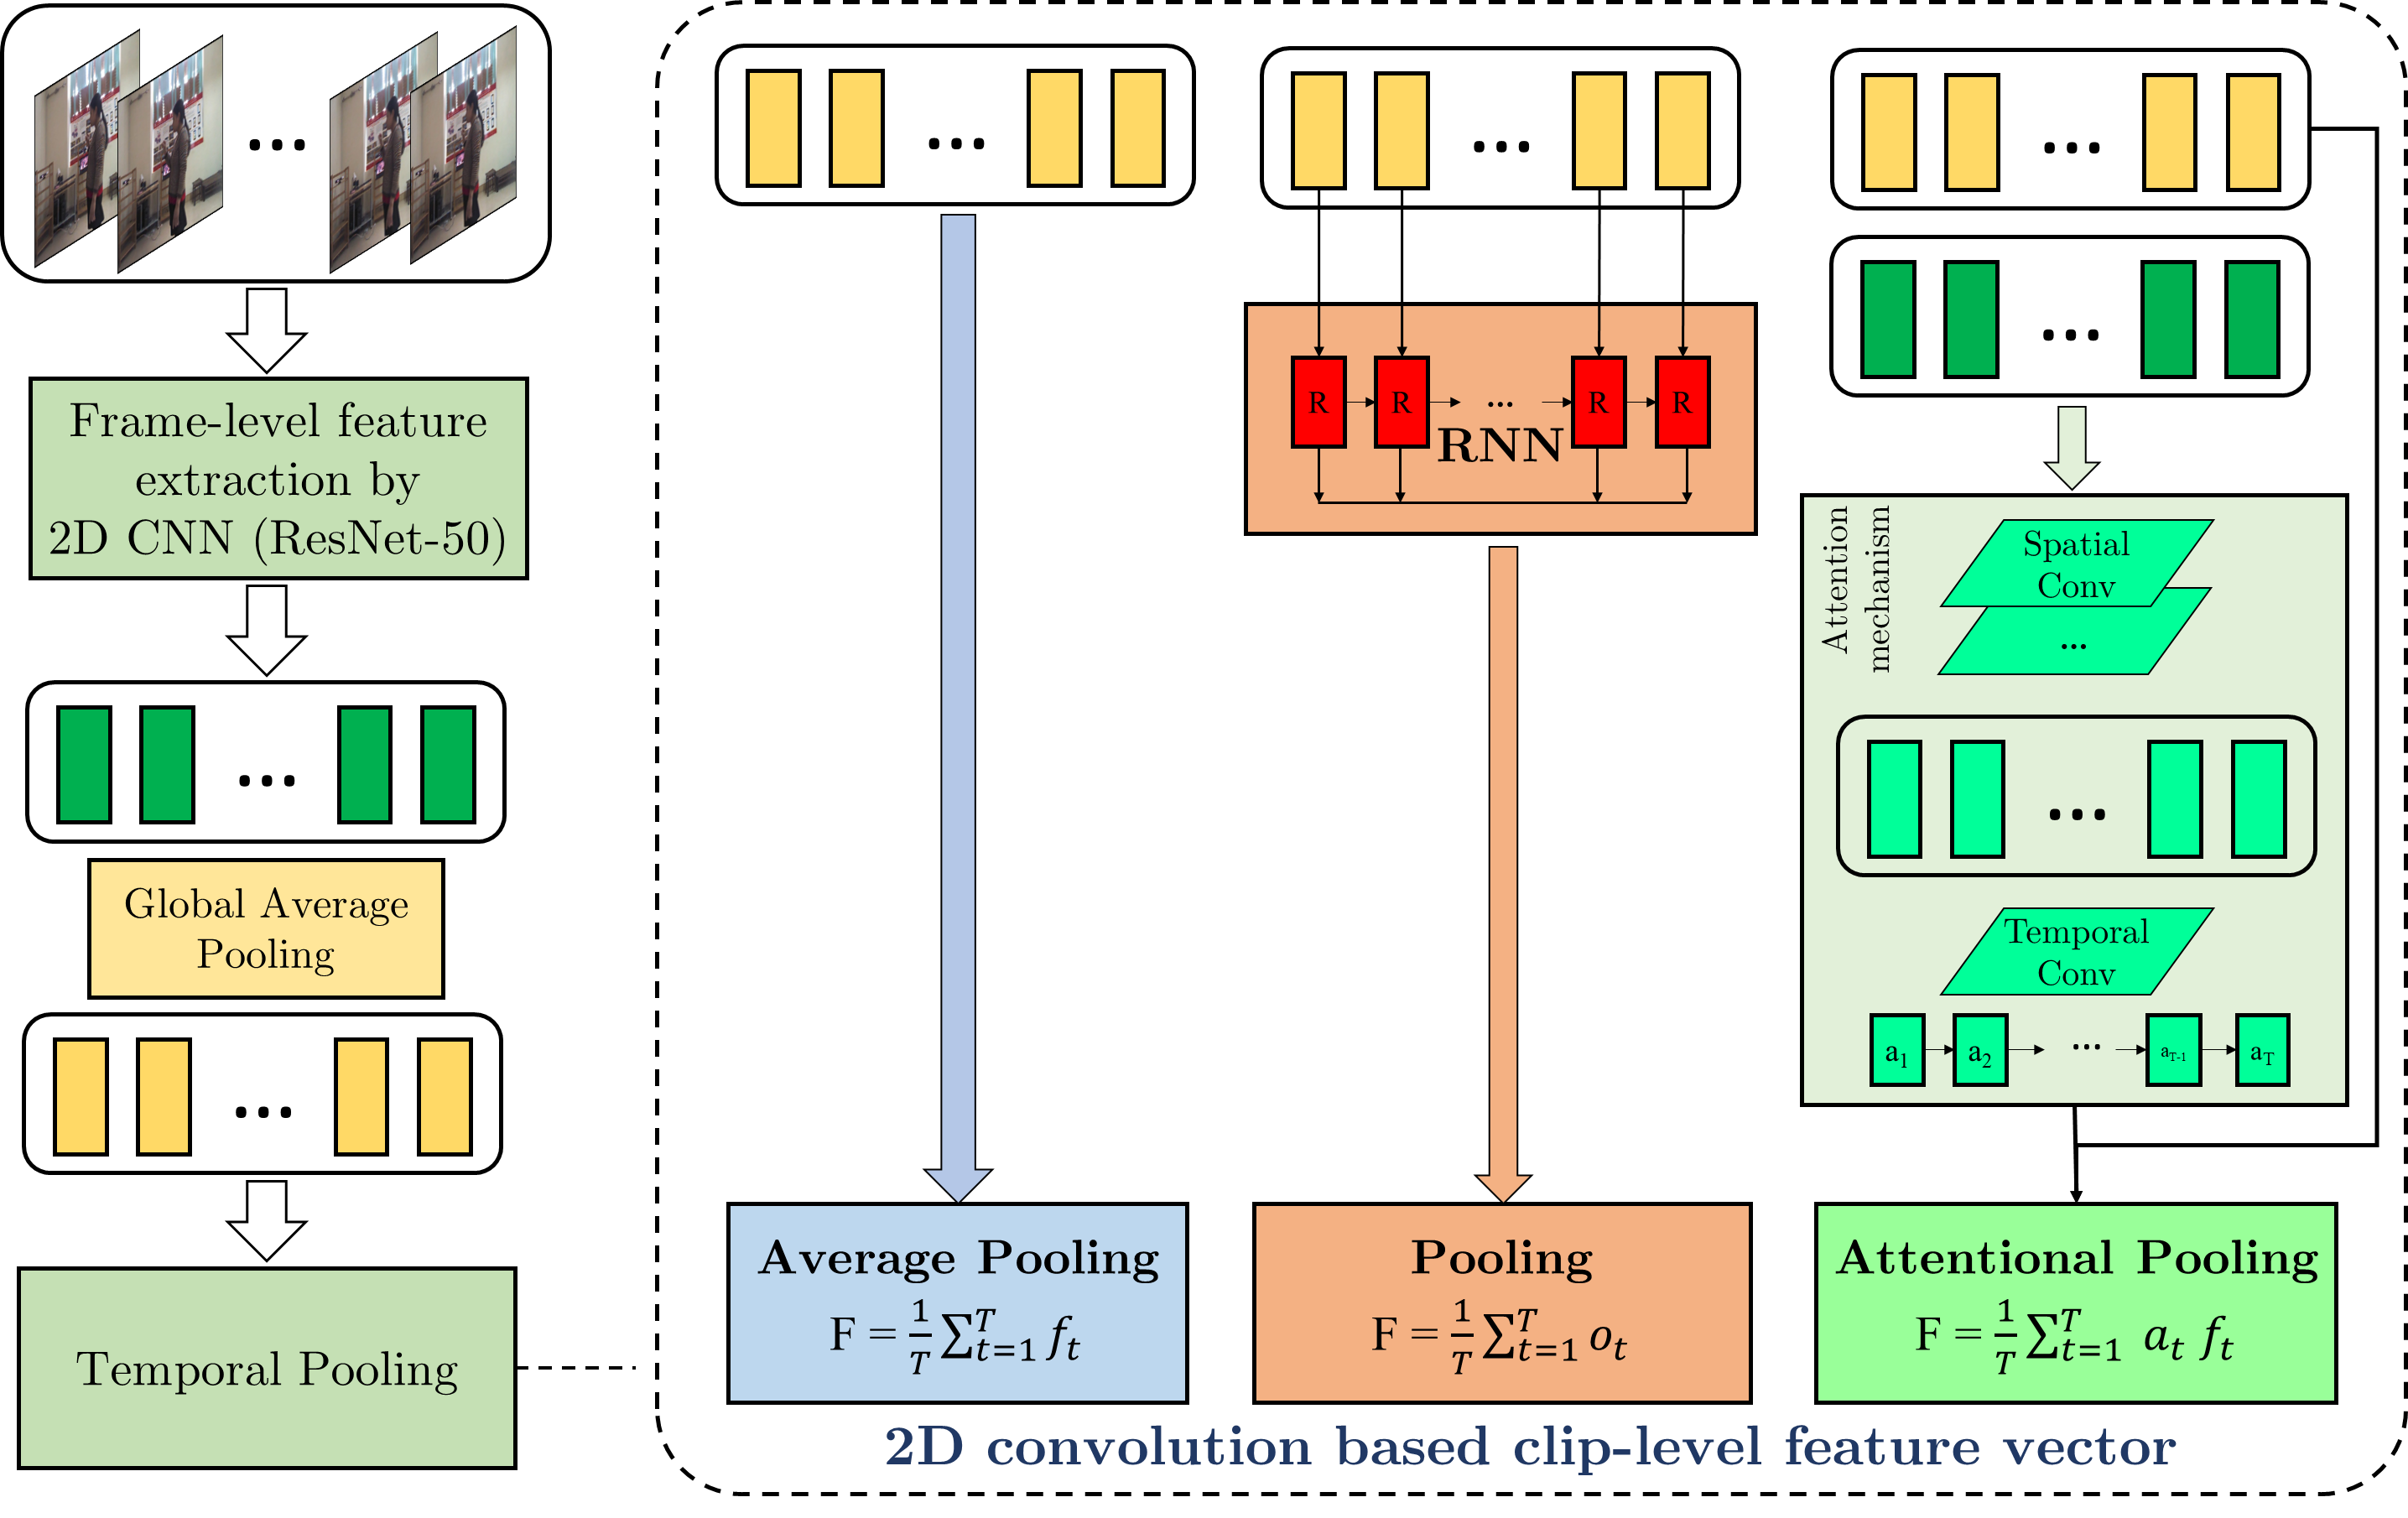
\includegraphics[width=1\linewidth]{figs/Pooling.png}
        \caption{Three pooling techniques: Average Pooling (AP), Recurrent Neural Network (RNN) and Temporal Attention Pooling (TA).}
        %\vspace{-0.3cm}
        \label{fig:pooling}
    \end{figure}

    \paragraph{Average Pooling - AP}: Let ${f}$ be the video-level feature, ${f_t}$ be the frame-level feature at time ${t}$, $T$ be the number of frames in video. Average pooling technique simply averages all frame-level features uniformly to create the video-level feature:
    \begin{equation}
        f=\frac{1}{T}\sum_{t=1}^T{f_t}
    \end{equation}
    As a frame-level feature is a 2048-D vector, the video-level feature is of same dimension.\\

    \paragraph{Recurrent Neural Network - RNN}: An RNN cell encodes a $t^{th}$ frame-level feature at time $t$ of the sequence and passes the hidden state $h_t$ into the next time step. The RNN is a single-layer with $T$ cells. In this work, the cell is LSTM (Long Short Term Memory). Each cell outputs a 512-D feature vector that contains information of the current frame and the previous ones. A sequence of frame-level features is aggregated into a video-level feature $f$ by calculating the average of the RNN outputs $o_t = R(f_t, o_{t-1})$; $t \in [1;T]$. 
    \begin{equation}
        f=\frac{1}{T}\sum_{t=1}^T{o_t}
    \end{equation}

    \paragraph{Temporal Attention - TA}: In the above pooling techniques, frame-level features are equally aggregated. In reality, some frames might have more important roles than remaining ones for recognizing an action. In temporal attention model, a weight $a_t$ is learnt for each frame $f_t$ and an attention weighted average is applied on the sequence of frame-level features as follows:
    \begin{equation}
        f=\frac{1}{T} \sum_{t=1}^{T}a_{t}f_{t}
    \end{equation}
    To learn the weights $a_t, t \in [1, T]$, the attention generation network proposed by Jiyang Gao et al. \cite{gao2018revisiting} is adopted. The network takes a sequence of frame-level features $[T, w, h, 2048]$, each is tensor extracted from the last convolution layer of ResNet-50. The network architecture consists of two main components: Spatial Convolution and Temporal Convolution. Firstly, a conv layer with shape $\{w, h, 2048, d_t\}$ is applied, then we get a $d_t$-dimensional feature for each frame of the clip ($d_t$ = input channel). A temporal conv layer $\{3, d_t, 1\}$ is then applied on these frame-level features to generate temporal attentions $s_c^t$. Once $s_c^t$ is obtained, the final attention score $a_t$ is computed by Softmax function:
    \begin{equation}
        a_t = \frac{e^{s_c^t}}{\sum_{k=1}^{T}e^{s_c^k}}
    \end{equation}
